% cSpell:language es,en
% ==================================================================
% CAPÍTULO 2: ESTADO DEL ARTE
% ==================================================================

\chapter{Estado del arte o de la cuestión, alternativas de solución al problema o desafío a resolver}

% ------------------------------------------------------------------
\section{Antecedentes de solución semejantes o similares al desafío de ingeniería}
% ------------------------------------------------------------------

\subsection{Sistemas de análisis visual con inteligencia artificial multimodal}

\subsubsection{Caso 1: GPT-4 Vision para análisis de objetos (OpenAI, Estados Unidos, 2023)}

GPT-4 Vision, lanzado en septiembre de 2023, representa el primer modelo de lenguaje de gran escala con capacidades multimodal nativas de OpenAI. El sistema demuestra capacidades avanzadas de interpretación visual con un 95\% de precisión en reconocimiento de objetos comunes y 78.5\% de efectividad en análisis de gráficos complejos según evaluaciones técnicas independientes \cite{ArticleRef255136}.

En términos de estimación dimensional, GPT-4V utiliza razonamiento contextual para comparar tamaños relativos entre objetos, empleando elementos conocidos como referencias de escala. Las evaluaciones técnicas reportan una precisión de $\pm$15--25\% de error en estimaciones dimensionales cuando se proporcionan referencias visuales adecuadas, mejorando a $\pm$10--20\% bajo condiciones de iluminación controlada \cite{Yu2024}.

\begin{figure}[H]
    \centering
    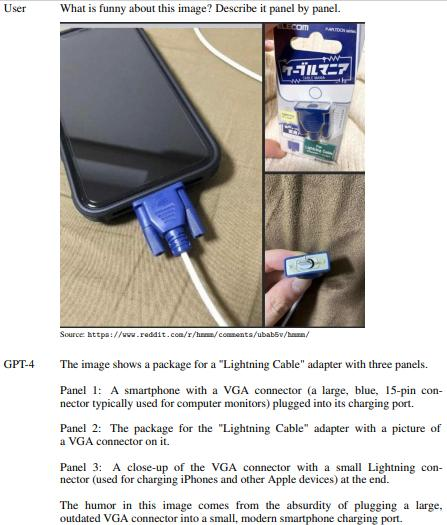
\includegraphics[width=0.9\textwidth]{gpt4_vision_example.png}
    \caption{Consulta a GPT-4 para análisis de múltiples imágenes. Fuente \cite{ArticleRef255134}}
    \label{fig:gpt4_vision}
\end{figure}

La arquitectura se basa en un \textit{transformer} multimodal que integra un codificador visual especializado con el modelo de lenguaje GPT-4, estimado en 1.76 trillones de parámetros. El sistema procesa imágenes de hasta 2048$\times$2048 píxeles en formatos JPEG, PNG, GIF y WebP, utilizando técnicas de atención cruzada para correlacionar información visual con conocimiento lingüístico \cite{ArticleRef255134}.

El modelo emplea un enfoque de \textit{vision-language understanding} que permite no solo identificar objetos, sino también razonar sobre sus propiedades físicas, relaciones espaciales y características dimensionales mediante una interpretación contextual similar al razonamiento humano \cite{ArticleRef255136}.

Las evaluaciones técnicas del sistema revelan un rendimiento variable según el contexto de aplicación:

\begin{itemize}
    \item MMMU \textit{Benchmark}: 56.8\% en tareas multimodal complejas
    \item \textit{MathVista}: 49.9\% en razonamiento visual-matemático
    \item AI2D: 78.2\% en interpretación de diagramas técnicos
    \item ChartQA: 78.5\% en análisis de gráficos y visualizaciones
\end{itemize}

Para tareas específicas de estimación dimensional, el sistema muestra mejor rendimiento en cajas rectangulares estándar, objetos con formas geométricas simples y productos comerciales conocidos, alcanzando precisiones útiles para la categorización logística y la clasificación de tarifas de envío \cite{Yu2024}.

Las evaluaciones técnicas identifican limitaciones significativas en aplicaciones que requieren precisión cuantitativa absoluta:

\begin{itemize}
    \item \textbf{Sin calibración externa:} incremento del error a $\pm$30--50\% en ausencia de referencias de escala conocidas.
    \item \textbf{Sensibilidad ambiental:} degradación de precisión con variaciones en iluminación, ángulos de captura y condiciones visuales.
    \item \textbf{Limitaciones de escala:} rendimiento reducido en objetos menores a 5\,cm o con formas irregulares complejas.
    \item \textbf{Objetos problemáticos:} dificultades con elementos transparentes, reflectivos o sin texturas distintivas.
\end{itemize}

El \textit{GPT-4V System Card} oficial de OpenAI reconoce explícitamente que “el modelo no está optimizado para mediciones precisas y puede proporcionar estimaciones aproximadas que requieren validación adicional para aplicaciones críticas” \cite{ArticleRef255136}.


\subsubsection{Caso 2: Claude 3 Vision}

Claude 3, lanzado en marzo de 2024 en sus variantes Haiku, Sonnet y Opus, establece un nuevo estándar en interpretación multimodal con un enfoque específico en razonamiento avanzado sobre contenido visual complejo. El sistema demuestra capacidades superiores a GPT-4V en interpretación de gráficos y documentos técnicos, alcanzando un 86.8\% en el benchmark MMLU y un 60.1\% en problemas matemáticos complejos con componentes visuales \cite{Anthropic2024}.

La arquitectura del modelo incorpora una ventana de contexto extendida de 200{,}000 tokens que incluye contenido visual, permitiendo el análisis simultáneo de múltiples imágenes y documentos dentro de una sola conversación. Esta capacidad es particularmente relevante para el análisis de inventarios complejos, donde se requiere correlacionar información entre múltiples fuentes visuales \cite{WebRef13251}.

\begin{figure}[H]
    \centering
    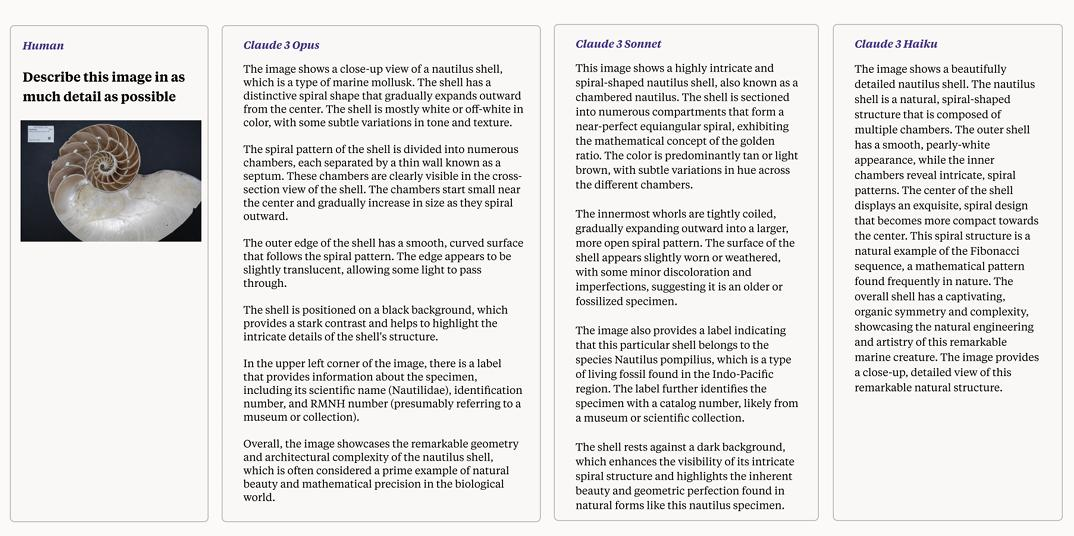
\includegraphics[width=0.85\textwidth]{claude3_vision_detection.png}
    \caption{Identificación de objetos visualmente usando modelos de Claude 3. Fuente: \cite{Anthropic2024}}
    \label{fig:claude3_detection}
\end{figure}

Claude 3 destaca en el reconocimiento óptico de caracteres (\textit{OCR}) en imágenes complejas, el procesamiento de documentos técnicos con \textit{layouts} sofisticados y la comprensión contextual de diagramas industriales, superando consistentemente a modelos anteriores en \textit{benchmarks} de comprensión documental \cite{Anthropic2024}.

El modelo exhibe capacidades avanzadas de razonamiento espacial que superan a sus predecesores en tareas que requieren comprensión de relaciones geométricas y propiedades físicas de objetos. Las evaluaciones técnicas independientes reportan un rendimiento superior en tareas de razonamiento espacial, con particular fortaleza en la interpretación de \textit{layouts} complejos y relaciones proporcionales entre elementos.

\begin{figure}[H]
    \centering
    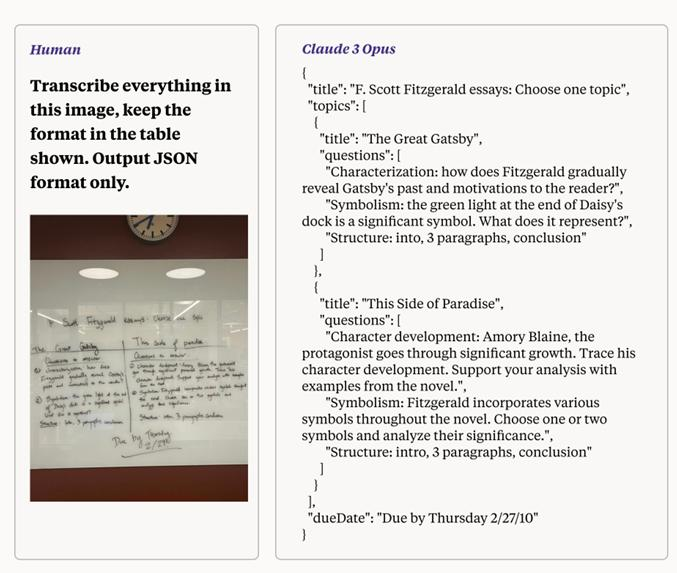
\includegraphics[width=0.85\textwidth]{claude3_json_output.png}
    \caption{Solicitud de reconocimiento de una imagen y reorganización en formato JSON.Fuente: \cite{Anthropic2024}}
    \label{fig:claude3_json}
\end{figure}

Para estimación dimensional, Claude 3 utiliza razonamiento contextual sofisticado que combina el reconocimiento de objetos conocidos con el análisis proporcional de elementos en la imagen. El sistema puede interpretar planos técnicos con dimensiones especificadas y extrapolar esta información para estimar las dimensiones de objetos fotografiados, logrando precisiones de $\pm$20--30\% en estimaciones sin referencias calibradas externas \cite{WebRef13251}.

La capacidad de procesamiento de documentos técnicos permite al modelo analizar especificaciones de productos, diagramas de embalaje y planos industriales, proporcionando estimaciones dimensionales basadas en la información contextual disponible en los documentos \cite{Anthropic2024}.

Claude 3 ofrece integración empresarial a través de la \textit{Anthropic API v1}, que proporciona \textit{endpoints RESTful} con autenticación basada en \textit{API keys} y límites de 4{,}000 tokens por minuto para todas las variantes del modelo. La \textit{API} soporta imágenes de hasta 20\,MB en formatos JPEG, PNG, GIF, WebP y PDF, facilitando la integración con sistemas existentes de gestión documental.

La arquitectura de la \textit{API} permite respuestas en múltiples formatos estructurados, incluyendo \textit{JSON}, texto estructurado y \textit{Markdown}, lo que facilita la integración con sistemas \textit{ERP}, plataformas de \textit{e-commerce} y aplicaciones de gestión logística. El sistema soporta procesamiento \textit{batch} para el análisis de grandes volúmenes de documentos y fotografías de inventario.

Las capacidades de \textit{streaming} permiten respuestas en tiempo real para aplicaciones interactivas, mientras que el modelo de \textit{pricing} por token de entrada y salida ofrece predictibilidad en los costos operacionales para implementaciones empresariales a gran escala.

Las implementaciones documentadas de Claude 3 en sectores logísticos y manufactureros incluyen aplicaciones específicas que aprovechan sus capacidades multimodales avanzadas:

\begin{itemize}
    \item \textbf{Análisis de especificaciones técnicas:} procesamiento automatizado de documentos de productos que incluyen planos técnicos con dimensiones especificadas, permitiendo extraer automáticamente información dimensional para sistemas de gestión de inventarios.
    \item \textbf{Interpretación de diagramas de embalaje:} análisis de documentos de \textit{packaging} que especifican configuraciones de empaque, permitiendo optimizar la utilización de espacio en contenedores y vehículos de transporte basándose en la interpretación visual de diagramas complejos.
    \item \textbf{Auditoría visual de inventarios:} procesamiento de fotografías de almacenes y centros de distribución para identificar discrepancias entre el inventario físico y los registros digitales, utilizando capacidades de reconocimiento de objetos y análisis espacial.
    \item \textbf{Análisis de documentos comerciales:} interpretación de facturas, órdenes de compra y documentos de envío que incluyen especificaciones de productos, automatizando la extracción de información dimensional crítica para procesos logísticos \cite{Anthropic2024}.
\end{itemize}

Las ventajas competitivas identificadas incluyen la ventana de contexto extendida (200K frente a 128K tokens de GPT-4), mejor comprensión de documentos complejos, razonamiento espacial más avanzado y menor tendencia a alucinaciones en datos técnicos críticos \cite{Anthropic2024}.

Las limitaciones operacionales incluyen una precisión dimensional comparable a GPT-4V ($\pm$20--30\%), dependencia de la calidad de imagen para un \textit{OCR} efectivo, costos por token potencialmente superiores a los de alternativas, y un ecosistema menos maduro de herramientas de terceros en comparación con OpenAI.


\subsubsection{Caso 3: Gemini 2.0 Flash}

Gemini 2.0 Flash, lanzado en diciembre de 2024, representa la segunda generación de modelos multimodales de Google con optimizaciones específicas para velocidad de procesamiento y análisis visual en tiempo real. El modelo incorpora una arquitectura \textit{transformer} multimodal de segunda generación optimizada para respuestas rápidas (denominación \textit{Flash}), logrando velocidades hasta 2$\times$ superiores a Gemini 1.0 en procesamiento multimodal \cite{Team20252, Team20251}.

El sistema soporta modalidades múltiples incluyendo texto, imagen, audio y video, con capacidad de procesamiento de imágenes de hasta 30\,MB en formatos \textit{JPEG}, \textit{PNG}, \textit{GIF}, \textit{WebP}, \textit{PDF}, \textit{SVG} y \textit{HEIC}. La ventana de contexto se expande masivamente a 2 millones de tokens, permitiendo el análisis simultáneo de múltiples documentos visuales complejos dentro de una sola sesión.

Las mejoras en análisis visual incluyen mejor razonamiento espacial, capacidades de análisis en tiempo real optimizadas y procesamiento simultáneo de hasta 20 objetos en una imagen individual, superando significativamente las limitaciones de 8--10 objetos de Gemini 1.0 \cite{Team20251}.


\begin{figure}[H]
    \centering
    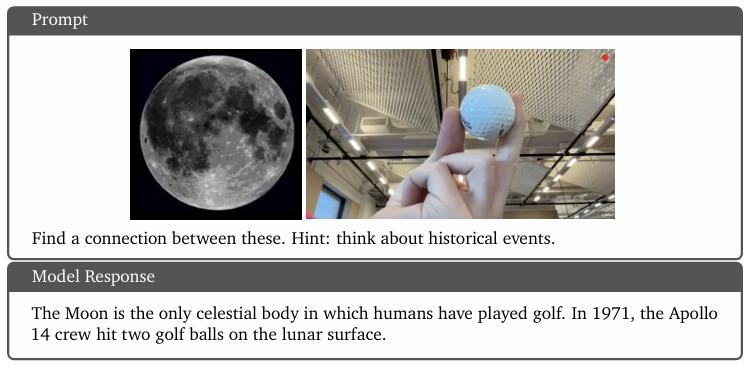
\includegraphics[width=0.9\textwidth]{gemini_multiimage_analysis.png}
    \caption{Se solicita a Gemini reconocer las imágenes y encontrar una relación entre ellas.}
    \label{fig:gemini_analysis}
\end{figure}

El sistema soporta modalidades múltiples incluyendo texto, imagen, audio y video, con capacidad de procesamiento de imágenes de hasta 30MB en formatos JPEG, PNG, GIF, WebP, PDF, SVG y HEIC. La ventana de contexto se expande masivamente a 2 millones de tokens.

Gemini 2.0 Flash integra Google Lens como módulo nativo, eliminando la arquitectura de integración externa de generaciones anteriores. El sistema demuestra precisión mejorada en estimaciones dimensionales, alcanzando márgenes de $\pm$8--15\% con objetos de referencia en productos estándar, $\pm$5--12\% en condiciones de laboratorio controlado, y $\pm$12--25\% en uso típico de usuarios reales \cite{Team20252}.

Implementaciones específicas en logística incluyen:
\begin{itemize}
    \item Análisis de inventario en tiempo real para Google Shopping
    \item Medición automatizada de productos para Google Merchant Center
    \item Optimización de embalaje en centros de distribución
    \item Análisis de fotografías de productos para Google Lens Shopping
\end{itemize}

\subsubsection{Caso 4: Vision Transformer (ViT) para reconocimiento y dimensionado de productos}

Vision Transformer (ViT), introducido por Dosovitskiy et al. en Google Research (2020) y publicado en ICLR 2021, revolucionó el campo de \textit{computer vision} al demostrar que arquitecturas transformer puras pueden superar las redes neuronales convolucionales tradicionales en tareas de reconocimiento de imágenes. El modelo alcanza 94.2\% de precisión en \textit{ImageNet classification} cuando se \textit{pre-entrena} en \textit{datasets} suficientemente grandes \cite{Dosovitskiy2020}.

La arquitectura divide imágenes en \textit{patches} de 16$\times$16 píxeles que se procesan como secuencias, similar al procesamiento de tokens en modelos de lenguaje. Esta metodología permite \textit{transfer learning} eficiente para nuevas categorías de productos.

Las implementaciones académicas posteriores han demostrado aplicabilidad directa en \textit{retail analytics}. DINOv2 (Meta AI Research, 2023) introduce \textit{self-supervised learning} que elimina la dependencia de datasets etiquetados masivos, logrando representaciones visuales robustas especialmente efectivas para reconocimiento de productos \cite{Oquab2024}.

Para estimación dimensional, las investigaciones académicas reportan precisiones de $\pm$12--18\% en objetos con referencias visuales, utilizando visual \textit{reasoning} sobre \textit{features transformer} que capturan relaciones espaciales complejas.

% ------------------------------------------------------------------
\subsection{Aplicaciones de LLMs multimodal en logística y comercio electrónico}
% ------------------------------------------------------------------

Florence (Microsoft Research, 2021) establece un framework multimodal que combina \textit{vision transformers} con capacidades de lenguaje natural, demostrando aplicabilidad directa para tareas que requieren comprensión semántica de productos y estimación de propiedades físicas.

Las evaluaciones académicas independientes confirman escalabilidad para procesamiento de millones de productos, con implementaciones que mantienen eficiencia computacional mediante técnicas de \textit{patch embedding} optimizadas.

% ------------------------------------------------------------------
\section{Características de soluciones semejantes o similares}
% ------------------------------------------------------------------

\subsection{Arquitecturas de procesamiento predominantes}

Las soluciones analizadas convergen en arquitecturas de procesamiento que combinan múltiples enfoques tecnológicos. Los sistemas comerciales líderes utilizan \textit{transformers} multimodal que integran vision encoders especializados (CLIP, ALIGN, ViT) con \textit{large language models} para interpretación semántica avanzada.

Las implementaciones actuales emplean \textit{attention mechanisms cross-modal} que permiten correlación directa entre características visuales y comprensión textual, facilitando estimación dimensional mediante razonamiento contextual \cite{Dosovitskiy2020}.

\subsection{Capacidades de interpretación dimensional}

Las capacidades de interpretación dimensional se fundamentan en:

\begin{enumerate}
    \item \textbf{Reconocimiento automático de referencias de escala}: Los modelos identifican objetos conocidos (monedas, tarjetas, manos humanas) para establecer proporciones relativas.
    \item \textbf{Análisis de perspectiva y profundidad visual}: Utiliza \textit{depth estimation} implícito derivado de características de textura y sombras.
    \item \textbf{Razonamiento contextual sofisticado}: Combina reconocimiento de objetos conocidos con análisis proporcional de elementos en la imagen \cite{Oquab2024}.
\end{enumerate}

\subsection{Precisión y confiabilidad según implementación}

La precisión varía significativamente según la implementación y condiciones operacionales:

\begin{table}[H]
\centering
\caption{Comparativa de precisión por tipo de sistema.}
\label{tab:precision_sistemas}
\begin{tabular}{@{}lcc@{}}
\toprule
\textbf{Tipo de Sistema} & \textbf{Condiciones Óptimas} & \textbf{Condiciones Reales} \\
\midrule
LLMs multimodal & $\pm$10--25\% & $\pm$15--30\% \\
Vision Transformers & $\pm$12--18\% & $\pm$15--25\% \\
Sistemas con hardware & $\pm$2--5mm & $\pm$5--10mm \\
\bottomrule
\end{tabular}
\end{table}

La degradación de precisión con iluminación deficiente, ángulos subóptimos y \textit{backgrounds} complejos representa un desafío común.

% ------------------------------------------------------------------
\section{Compendio de tecnologías, herramientas, métodos, modelos utilizados con éxito}
% ------------------------------------------------------------------

\subsection{Modelos de lenguaje multimodal predominantes}

\textbf{Modelos de gran escala comerciales:}
\begin{itemize}
    \item GPT-4 Vision (OpenAI) - 1.76 trillones de parámetros
    \item Claude Sonnet 4 (Anthropic) - Optimizado para razonamiento visual
    \item Gemini 2.0 Flash (Google) - Optimizaciones de velocidad
    \item LLaVA - Alternativas \textit{open-source}
\end{itemize}

\textbf{Arquitecturas especializadas predominantes:}
\begin{itemize}
    \item CLIP (\textit{Contrastive Language-Image Pre-training})
    \item BLIP-2 (\textit{Bootstrapped vision-language pre-training})
    \item InstructBLIP - Seguimiento de instrucciones específicas
    \item MiniGPT-4 - Eficiencia en recursos limitados
\end{itemize}

\subsection{Frameworks de visión por computadora académicos}

Vision Transformers (ViT) representan el estado del arte en análisis visual académico:

\begin{itemize}
    \item ViT-Base: 86 millones de parámetros
    \item ViT-Large: 307 millones de parámetros
    \item ViT-Huge: 632 millones de parámetros
\end{itemize}

Modelos híbridos incluyen DeiT (\textit{Data-efficient image Transformers}), Swin Transformer optimizado para imágenes de alta resolución, y EfficientViT diseñado para implementaciones móviles.

\subsection{Tecnologías de infraestructura en la nube}

\textbf{Plataformas de IA como servicio:}
\begin{itemize}
    \item OpenAI API con GPT-4 Vision endpoints
    \item Anthropic Claude API para análisis multimodal
    \item Google Vertex AI con modelos Gemini integrados
    \item Azure Cognitive Services
    \item AWS Bedrock
\end{itemize}

\textbf{Servicios de computación distribuida:}
\begin{itemize}
    \item AWS Lambda - Procesamiento \textit{serverless}
    \item Google Cloud Run - Containerización
    \item Azure Container Instances - Escalabilidad elástica
    \item Kubernetes - Orquestación de microservicios
\end{itemize}

\subsection{Herramientas de desarrollo e integración}

\textbf{Bibliotecas de integración:}
\begin{itemize}
    \item LangChain - Framework para aplicaciones LLM
    \item LlamaIndex - \textit{Retrieval-Augmented Generation}
    \item Haystack - Pipelines \textit{end-to-end}
    \item Transformers (HuggingFace) - Acceso a modelos pre-entrenados
\end{itemize}

\textbf{SDKs para desarrollo móvil:}
\begin{itemize}
    \item React Native con plugins para APIs de IA
    \item Flutter con packages para computer vision
    \item Swift/Kotlin con SDKs nativos
    \item Progressive Web Apps para acceso universal
\end{itemize}

\subsection{Metodologías de prompt engineering y optimización}

\textbf{Técnicas avanzadas de diseño de prompts:}
\begin{itemize}
    \item \textit{Few-shot learning} para medición dimensional
    \item \textit{Chain-of-thought prompting} para razonamiento paso a paso
    \item \textit{Structured output formatting} para consistencia
    \item \textit{Multi-turn conversation} para refinación iterativa
\end{itemize}

\textbf{Estrategias de optimización:}
\begin{itemize}
    \item \textit{Fine-tuning} con datos del dominio logístico
    \item \textit{Retrieval-Augmented Generation} (RAG)
    \item \textit{In-context learning} con ejemplos calibrados
    \item LoRA y Adapters para personalización eficiente
\end{itemize}

% ------------------------------------------------------------------
\section{Conjunto de características y especificaciones para la solución óptima}
% ------------------------------------------------------------------

\subsection{Arquitectura tecnológica óptima}

Basándose en el análisis de soluciones existentes, la arquitectura óptima debe combinar:

\begin{itemize}
    \item Modelos de lenguaje multimodal de última generación
    \item Infraestructura \textit{cloud} escalable
    \item Procesamiento distribuido eficiente
    \item Interfaces móviles intuitivas
\end{itemize}

\subsection{Precisión y confiabilidad requeridas}

Para aplicaciones logísticas comerciales, el sistema debe alcanzar:

\begin{itemize}
    \item Precisión de $\pm$15--20\% en condiciones reales de uso
    \item Mejora a $\pm$10--15\% con referencias de escala adecuadas
    \item Tiempos de respuesta inferiores a 5 segundos
    \item Disponibilidad superior al 99.5\%
\end{itemize}

Esta precisión es suficiente para categorización de tarifas de envío, optimización básica de carga vehicular, y estimaciones de costos logísticos sin requerir inversión en hardware especializado.

\subsection{Limitaciones y alcances reconocidos}

El sistema está diseñado para:

\begin{itemize}
    \item Estimaciones dimensionales aproximadas para categorización logística
    \item Paquetes regulares de e-commerce (5cm a 2 metros)
    \item Condiciones de iluminación mínima adecuada
    \item Mercado peruano inicialmente, con escalabilidad regional
\end{itemize}

Limitaciones reconocidas:

\begin{itemize}
    \item No apto para aplicaciones que requieran precisión milimétrica
    \item Degradación con objetos transparentes o altamente reflectivos
    \item Requiere iluminación mínima adecuada
    \item Formas extremadamente irregulares presentan mayor error
\end{itemize}